\documentclass[12pt, a4paper]{article}
\usepackage[scaled]{helvet}
\renewcommand\familydefault{\sfdefault}
\usepackage[T1]{fontenc}
\usepackage[margin=0.5in]{geometry}
\usepackage{float}
\usepackage{framed}
\usepackage{multicol}
\usepackage{amsmath}
\usepackage[framemethod=TikZ]{mdframed}
\usepackage{graphicx}
\usepackage{enumitem}
\setlist{nosep}

\newcounter{note}\setcounter{note}{0}
\renewcommand{\thenote}{\arabic{note}}
\newenvironment{note}[1]{
	\stepcounter{note}
	\ifstrempty{#1}{
		\mdfsetup{
			frametitle={
				\tikz[baseline=(current bounding box.east),outer sep=0pt]
				\node[anchor=east,rectangle,fill=blue!20]
				{\strut Note~\thenote};
			}
		}
	}{
		\mdfsetup{
			frametitle={
				\tikz[baseline=(current bounding box.east),outer sep=0pt]
				\node[anchor=east,rectangle,fill=blue!20]
				{\strut Note~\thenote:~#1};
			}
		}
	}
	\mdfsetup{innertopmargin=0pt,linecolor=blue!20,linewidth=2pt,topline=true,frametitleaboveskip=\dimexpr-\ht\strutbox\relax}
	\begin{mdframed}[]\relax
}{
	\end{mdframed}
}

\begin{document}
	\tableofcontents
	\vspace{2em}
	\textbf{Contributors:}
	\begin{itemize}
		\item Daniel Fitz (Sanchez)
	\end{itemize}
	
	\section{Sem Outline}
	\begin{table}[H]
		\begin{tabular}{ll}
			Week (dates) & Lecture\\
			1 & Computer Networks and the Internet\\
			2 & Principles of Nw Apps: HTTP, SMTP, DNS\\
			3 & Application Layer: P2P, CDN, Sockets\\
			4 & Networking at UQ\\
			5 & Transport Layer: UDP\\
			6 & Transport Layer: TCP\\
			7 & Network Layer: Data Plane\\
			8 & Network Layer: Control Place\\
			9 & Link Layer\\
			11 & Wireless and Mobile\\
			12 & Security\\
			13 & Multimedia
		\end{tabular}
		\centering
		\caption{Week Outline}
	\end{table}


\newpage
\begin{multicols*}{2}
	
	\section{Lecture 1}
	\begin{itemize}
		\item billions of connected computing devices
		\item transmission rate: \textbf{bandwidth}
		\item \textbf{Packet Switches:} Forward packets
		\begin{itemize}
			\item \textbf{routers} and \textbf{switches}
		\end{itemize}
		\item \textbf{Internet: ``network of networks''} (Interconnected ISPs)
		\item \textbf{Protocols} control sending, receiving (e.g. TCP, IP, HTTP, Skype, 802.11)
		\item \textbf{Internet standards}
		\begin{description}
			\item[RFC:] Request for comments
			\item[IETF:] Internet Engineering Task Force
		\end{description}
	\end{itemize}

\subsection{Network Structure}
\begin{itemize}
	\item \textbf{Network Edge}
	\begin{itemize}
		\item hosts: clients and servers
		\item servers often in data centers
	\end{itemize}
	\item \textbf{Access networks, physical media:} wired, wireless communication links
	\item \textbf{network core:}
	\begin{itemize}
		\item interconnected routers
		\item network of networks
	\end{itemize}
\end{itemize}

\subsection{Access Network}
\subsubsection{Digital Subscriber Line (DSL)}
\begin{itemize}
	\item use \textbf{existing} telephone line to central office DSLAM
	\begin{itemize}
		\item data over DSL phone line goes to Internet
		\item voice over DSL phone line goes to telephone net
	\end{itemize}
	\item < 2.5 Mbps upstream transmission rate (typically < 1 Mbps)
	\item < 24 Mbps downstream transmission rate (typically < 10 Mbps)
\end{itemize}
\subsubsection{Cable Network}
\begin{leftbar}
	\textbf{frequency division multiplexing:} different channels transmitted in different frequency bands
\end{leftbar}
\begin{itemize}
	\item \textbf{HFC: hybrid fiber coax}
	\begin{itemize}
		\item asymmetric: up to 30Mbps downstream transmission rate, 2 Mbps upstream transmission rate
	\end{itemize}
	\item \textbf{network} of cable, fiber attaches homes to ISP router
	\begin{itemize}
		\item homes \textbf{share access network} to cable head-end
		\item unlike DSL, which has dedicated access to central office
	\end{itemize}
\end{itemize}
	\textbf{wireless LANS:}
	\begin{itemize}
		\item within building (30 meters)
		\item 802.11b/g/n (WiFi): 11,54,450 Mbps transmission rate
	\end{itemize}
	\textbf{wide-area wireless access:}
	\begin{itemize}
		\item provided by telco (cellular) operator, 10's km
		\item between 1 and 10 Mbps
		\item 3G, 4G, LTE
	\end{itemize}

\subsection{Sending}
\begin{itemize}
	\item takes application message
	\item breaks into smaller chunks, known as \textbf{packets}, of length \textbf{$L$} bits
	\item transmites packet into access network at \textbf{transmission rate $R$}
	\begin{itemize}
		\item link transmission rate, aka link \textbf{capacity, aka link bandwidth}
	\end{itemize}
\end{itemize}
\begin{note}{Packet Transmission Delay}
	\[
		\text{\parbox{2cm}{packet transmission delay}}=\text{\parbox{2cm}{time needed to transmit $L$-bit packet into link}}=\frac{L\text{ (bits)}}{R\text{ (bits/sec)}}
	\]
\end{note}

\subsection{Physical Media}
\begin{itemize}
	\item \textbf{bit:} propagates between transmitter/receiver pairs
	\item \textbf{physical link:} what lies between transmitter and receiver
	\item \textbf{guided media:} signals propagate in solid media (copper, fiber, coax)
	\item \textbf{unguided media:} signals propagate freely, e.g. radio
	\item \textbf{twisted pair (TP):} two insulated copper wires
	\begin{itemize}
		\item Category 5: 100 Mbps, 1 Gbps Ethernet
		\item Category 6: 10 Gbps
	\end{itemize}
\end{itemize}
\subsubsection{Coax}
\begin{itemize}
	\item two concentric copper conductors
	\item bidirectional
	\item broadband: multiple channels on cable, HFC
\end{itemize}
\subsubsection{Fiber Optic Cable}
\begin{itemize}
	\item glass fiber carrying light pulses, each pulse a bit
	\item high-speed operation: high-speed point-to-point transmission (e.g. 10's - 100's Gbps transmission rate)
	\item low error rate
	\begin{itemize}
		\item repeaters spaced far apart
		\item immune to electromagnetic noise
	\end{itemize}
\end{itemize}
\subsubsection{Radio}
\begin{itemize}
	\item signal carried in electromagnetic spectrum
	\item no physical "wire"
	\item bidirectional
	\item propagation environment effects:
	\begin{itemize}
		\item reflection
		\item obstruction by objects
		\item interference
	\end{itemize}
\end{itemize}
\textbf{Radio Link Types:}
\begin{itemize}
	\item \textbf{terrestrial microwave:} up to 45 Mbps channels
	\item \textbf{LAN} (e.g. WiFi) 54 Mbps
	\item \textbf{wide-area} (e.g. cellular) 4G cellular: \~ 10 Mbps
	\item \textbf{satellite}
	\begin{itemize}
		\item Kbps to 45 Mbps channel (or multiple smaller channels)
		\item 270 msec end-end delay
		\item geosynchronous versus low altitude
	\end{itemize}
\end{itemize}

\subsection{Packet-switching}
\subsubsection{Store-and-forward}
\begin{leftbar}
	$L$ bits per packet\\
	Source to destination: $R$ bps
\end{leftbar}
\begin{itemize}
	\item takes $\frac{L}{R}$ seconds to transmit (push out) $L$-bit packet into link at $R$ bps
	\item \textbf{store and forward:} entire packet must arrive at router before it can be transmitted on next link
\end{itemize}
\begin{note}{End-End delay}
	\[
		\text{delay} = 2\frac{L}{R}
	\]
	(assuming zero propagation delay)
\end{note}
\subsubsection{Packet switching versus circuit switching}
Is packet switching a ``slam dunk winner?''
\begin{itemize}
	\item great for bursty data (resource sharing, simpler, no call setup)
	\item excessive congestion possible: packet delay and loss (protocols needed for reliable data transfer, congestion control)
\end{itemize}

\subsection{Packet Loss}
\begin{figure}[H]
	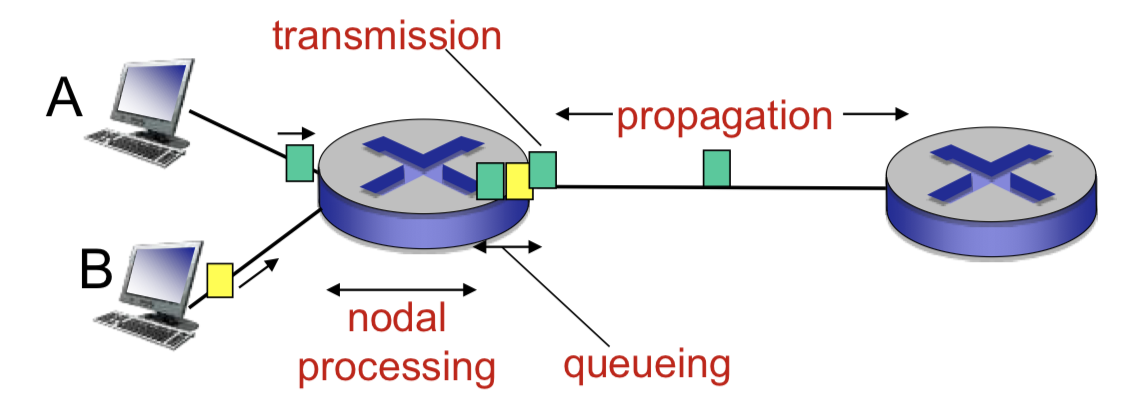
\includegraphics[width=8cm]{delay}
	\centering
	\caption{Packet Delay Algorithm Explanation}
\end{figure}
\begin{note}{Packet Delay Algorithm}
	\[ d_\text{nodal} = d_\text{proc} + d_\text{queue} + d_\text{trans} + d_\text{prop} \]
\end{note}
\subsubsection{Nodal Processing}
\[ d_\text{proc} \]
\begin{itemize}
	\item check bit errors
	\item determine output link
	\item typically < msec
\end{itemize}
\subsubsection{Queuing Delay}
\[ d_\text{queue} \]
\begin{itemize}
	\item time waiting at output link for transmission
	\item depends on congestion level of router
\end{itemize}
\subsubsection{Transmission Delay}
\[ d_\text{trans} \]
\begin{itemize}
	\item $L$: packet length (bits)
	\item $R$: link bandwidth(bps)
	\item $d_\text{trans} = \frac{L}{R}$
\end{itemize}
\subsubsection{Propagation Delay}
\[ d_\text{prop} \]
\begin{itemize}
	\item $d$: length of physical link
	\item $s$: propagation speed ($\approx2\times10^8$ m/sec)
	\item $d_\text{prop} = \frac{d}{s}$
\end{itemize}

\subsection{Throughput}
\begin{leftbar}
	Rate (bits/time unit) at which bits transferred between sender/receiver
\end{leftbar}
\begin{description}
	\item[Instantaneous:] rate at given point in time
	\item[Average:] rate over longer period of time
\end{description}
\begin{note}{Bottleneck Link}
	Link on end-end path that constrains end-end throughput
\end{note}

\subsection{Layering}
\subsubsection{Why Layering?}
Dealing with complex systems:
\begin{itemize}
	\item Explicit structure allows identification, relationship of complex system's pieces (layered \textbf{reference model} for discussion)
	\item Modularization eases maintenance, updating system
	\begin{itemize}
		\item change of implementation of layer's service transparent to rest of system
		\item e.g. change in gate procedure doesn't affect rest of system
	\end{itemize}
	\item layering considered harmful?
\end{itemize}
\subsubsection{Internet Protocol Stack}
\begin{description}
	\item[Application:] supporting network applications (FTP, SMTP, HTTP)
	\item[Transport:] process-process data transfer (TCP, UDP)
	\item[Network:] routing of datagrams from source to destination (IP, routing protocols)
	\item[Link:] data transfer between neighboring network elements (Ethernet, 802.111 (WiFi), PPP)
	\item[Physical:] bits ``on the wire''
\end{description}
\subsubsection{ISO/OSI Reference Model}
Internet stack ``missing'' these layers. These services, if needed, must be implemented in application.
\begin{description}
	\item[Application:]
	\item[Presentation:] allow applications to interpret meaning of data, e.g. encryption, compression, machine-specific conventions
	\item[Session:] synchronization, check-pointing, recovery of data exchange
	\item[Transport:]
	\item[Network:]
	\item[Link:]
	\item[Physical:]
\end{description}

\subsection{Security}
\begin{itemize}
	\item Malware can get in host from:
	\begin{description}
		\item[Virus:] self-replicating infection by receiving/executing object (e.g. e-mail attachment)
		\item[Worm:] self-replicating infection by passively receiving object that gets itself executed
	\end{description}
	\item \textbf{Spyware malware} can record keystrokes, web sites visited, upload info to collection site
	\item Infected host can be enrolled in \textbf{botnet}, used for spam. DDoS attacks
\end{itemize}
\subsubsection{DoS: Denial of Service}
\textbf{Denial of Service (DoS):} attackers make resources (server, bandwidth) unavailable to legitimate traffic by overwhelming resource with bogus traffic
\begin{enumerate}
	\item select target
	\item break into hosts around the network (botnet)
	\item send packets to target from compromised hosts
\end{enumerate}
\subsubsection{Sniffing}
\begin{itemize}
	\item broadcast media (shared Ethernet, wireless)
	\item promiscuous network interface reads/records all packets (e.g. including passwords) passing by
\end{itemize}
\subsubsection{IP Spoofing}
Send packet with false source address


\end{multicols*}	
\end{document}